\chapter{Análise de resultados}
 O objetivo do projeto era o desenvolvimento de uma aplicação mobile com foco na área de forum da mesma, devendo este permitir o registo de empresas, gestão de utilizadores pelas mesmas, notificações, comunicações por email, gestão de conta e notificações do utilizador.

 \section{Tarefas}

A nível de tarefas o esperado, como mencionado no capítulo \ref{sec:planificacao trabalho}, seria terminar o projeto no final de março, o que não se tornou realidade devido a diversos imprevistos que ocorreram no caminho, sendo o principal imprevisto o atraso no desenvolvimento do webscraper, devido à constante atualização do catálogo o que levava a alterações no conteúdo do website sendo assim necessário alterar o código de leitura do mesmo a cada alteração. Outro grande problema encontrado foi a alteração de alguns requisitos durante o desenvolvimento, o que levava a mais tarefas e por si mais tempo de desenvolvimento.

Estes imprevistos e dificuldades no desenvolvimento levaram a um atraso no desenvolvimento da aplicação em 1 mês e 1 semana, sendo assim estava previsto o término em março tendo a aplicação sido terminada no início de maio.

Apesar de todas as dificuldades todas as tarefas previstas foram concluídas não existindo assim funcionalidades por implementar.

\begin{figure}[htb]
  \centering
  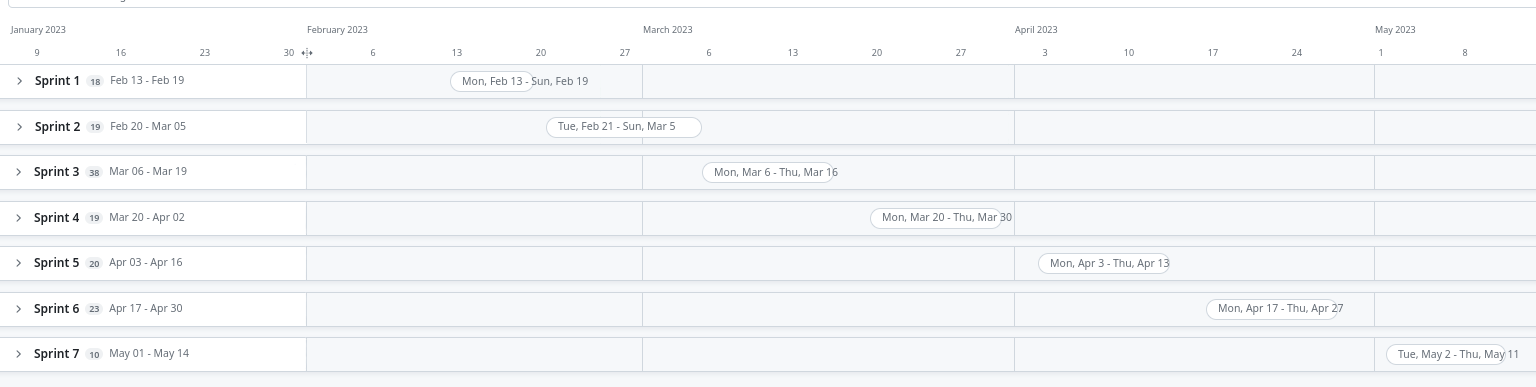
\includegraphics[width=\textwidth]{images/analise_resultados/planeamento_final.png}
  \caption{Organização de tarefas final}
  \label{fig:77}
\end{figure}

\newpage

\section{Base de dados}

Um dos pontos que sofreu mais alterações durante o desenvolvimento do projeto foi a base de dados, pois com alteração de requisitos e de catálogo de produtos foram necessárias realizar várias alterações até alcançar a versão final.

\begin{figure}[htb]
  \centering
  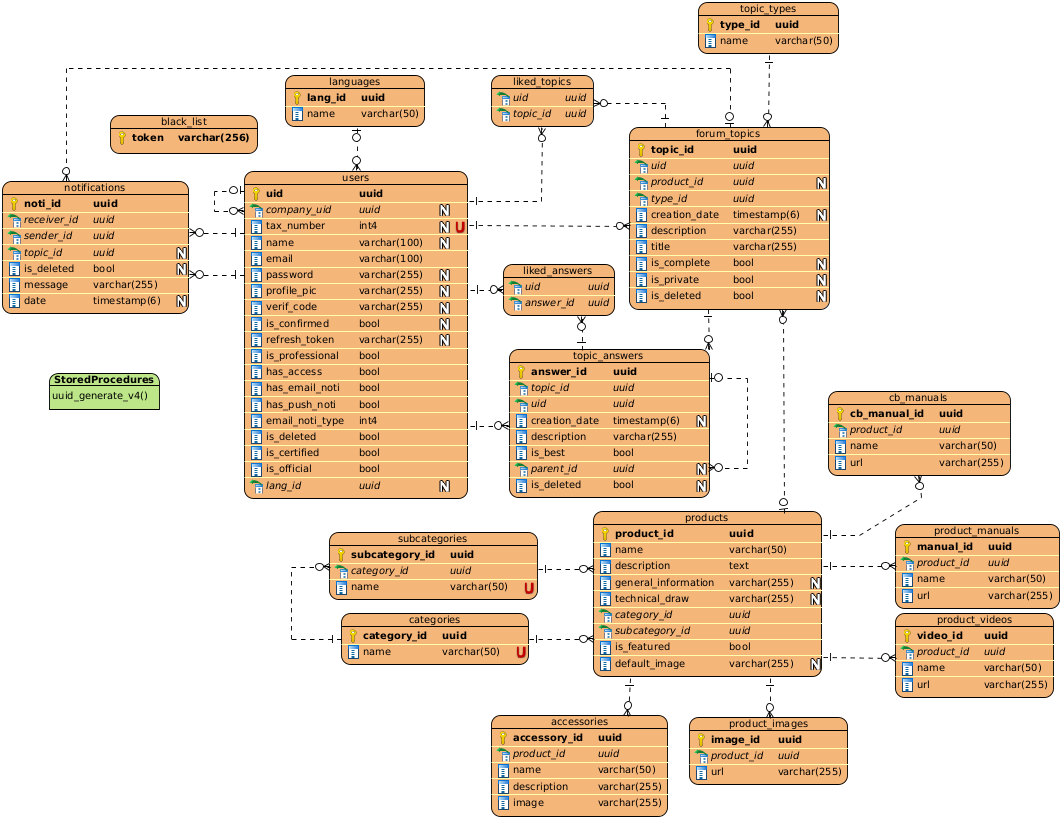
\includegraphics[width=0.7\textwidth]{images/diagramas/diagrama_bd.png}
  \caption{Base de dados inicial}
  \label{fig:78}
\end{figure}

\begin{figure}[htb]
  \centering
  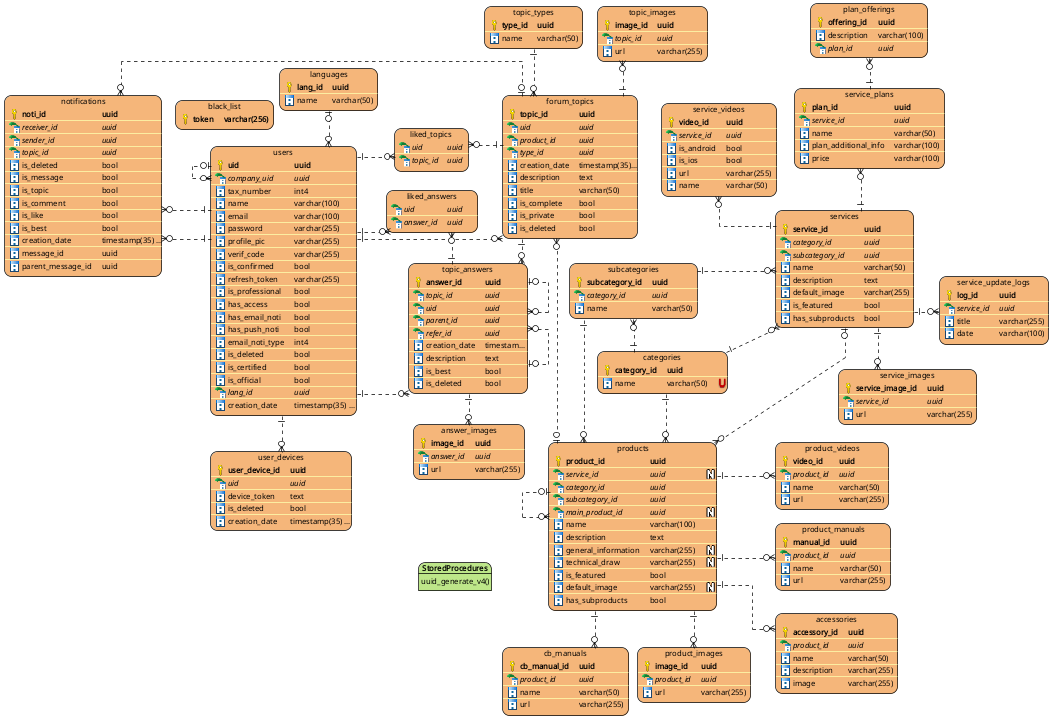
\includegraphics[width=0.7\textwidth]{images/diagramas/bd_final.png}
  \caption{Base de dados final}
  \label{fig:79}
\end{figure}

\section{Opinião do cliente}

Após o desenvolvimento do projeto este foi apresentado ao cliente de forma a verificar se este se encontrava de acordo com os requisitos e expectativas do mesmo.

Após a apresentação, o cliente, dispôs de uma opinião positiva, indicando que a aplicação encontra-se de acordo com as expectativas e requisitos, apenas faltando a testagem da mesma em relação a erros e performance, sendo que esta só poderia ser realizada uma vez que a aplicação seja lançada, sendo que seria necessário os utilizadores indicarem os erros.